\chapter{Introduction}
In this chapter, I provide the motivation for this project (\S\ref{sec:motive}) and setup the problem I am solving (\S\ref{sec:aim}). I also explain some key algorithms involved. Finally, I cover some related work (\S\ref{sec:relate}).
\section{Motivation}
\label{sec:motive}
Transmission Control Protocol (TCP) is the protocol of choice in many data centres. However, it is very sensitive to losses (by design, as a mean for congestion control), which can significantly degrade the performance within the data centres \cite{zilberman2017has}. Congestion control, avoidance and recovery mechanisms are thus of high importance in this field, and a lot of work has been done trying to minimise such loss rate. Still, not all TCP losses are born equal. For example, losses happening at the destination host’s network interface card (NIC) are not an indication of congestion within the network. It is assumed that fast retransmission of such lost packets, from within the network, can increase the utilisation of the network.

In-network computing, on the other hand, is an emerging research area in systems and networking, where applications traditionally running on the host are offloaded to the network hardware (e.g. switch, NIC). Examples of applications offloaded in the past include network functions (DNS server \cite{dns}), distributed systems functions such as consensus (P4xos \cite{p4xos, dang16}), coordination services for modern cloud systems (NetChain \cite{netChain}) and even a game (Tic-Tac-Toe). Key-Value Store (KVS) caching (NetCache \cite{netCache}) is also among the popular type of in-network applications. The main promises of in-network computing are performance, both in terms of throughput and latency, and power efficiency \cite{sigarch}.
  
Therefore, in this dissertation, I explore the possibility of applying network-accelerated KVS concepts to TCP fast retransmit mechanism in order to improve cross-datacentre performance. The scope of this project lies at the intersection of computer networking, cloud computing and programmable hardware design. Thus, its success would contribute towards those areas, especially data centre networks, where low latency and high data rate are desirable.

 \section{Project Aims}
 \label{sec:aim}
 A TCP sender normally uses retransmission timeout (RTO)—a simple timer—to recognise and retransmit lost segments. When TCP sends a segment, the timer starts and stops when the acknowledgement is received. If an acknowledgement is not received for a particular segment within a specified time (a function of the estimated round-trip delay time), the sender will assume the segment was lost in the network, and will retransmit the segment.
 
Fast retransmit is an enhancement to TCP that reduces the time a sender waits before retransmitting a lost segment. Duplicate acknowledgement (DUP ACK) is the basis for the fast retransmit mechanism. After receiving a packet (e.g. with sequence number 1), the receiver sends an acknowledgement by adding 1 to the sequence number (i.e. acknowledgement number 2). This indicates to the sender that the receiver received the packet number 1 and it expects packet number 2. Suppose that two subsequent packets are lost. The next packets the receiver sees are packet numbers 4 and 5. After receiving packet number 4, the receiver sends an acknowledgement, but still only for sequence number 2. When the receiver receives packet number 5, it sends yet another acknowledgement value of 2. DUP ACK occurs when the sender receives more than one acknowledgement with the same sequence number (2 in our example).

DUP ACKs are a sign of an isolated loss. The lack of acknowledgement number progress means 2 hasn’t been delivered, but the stream of ACKs means some packets are being delivered (4 and 5 in our example). When a sender receives several DUP ACKs, it can be reasonably confident that the segment with the sequence number specified in the DUP ACK was dropped. A sender with fast retransmit will then retransmit this packet immediately for the retransmission timer to expire.

\begin{figure}[h]
	\centering
	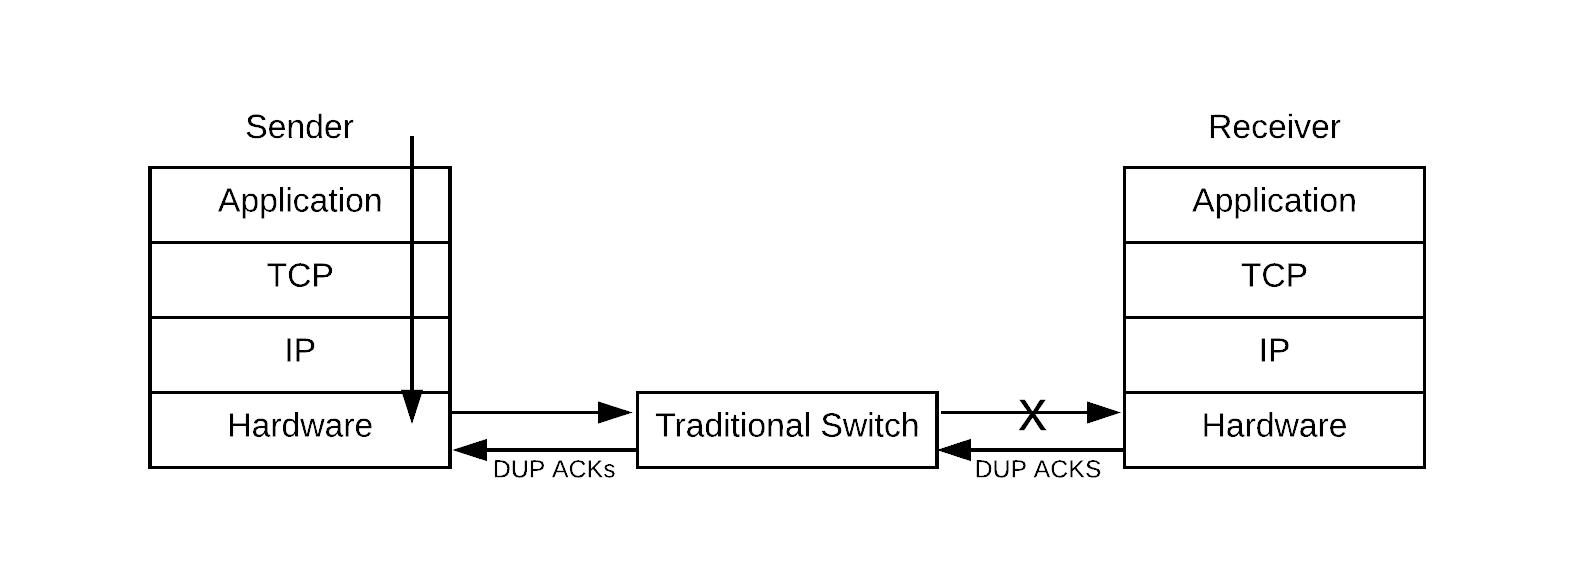
\includegraphics[width=\textwidth]{tradition-tcp.png}
	\caption{The standard convention of TCP fast retransmit.}
	\label{fig:tradition-tcp}
\end{figure}

Currently, the DUP ACKs will traverse all the way back to the sender (Figure \ref{fig:tradition-tcp}). The sender receives the DUP ACKs, then retransmits the packet with the next higher sequence number. In a typical data centre network, a packet will traverse multiple hops, so the delay induced by the network and the host is indeed substantial.

\begin{figure}[h]
	\centering
	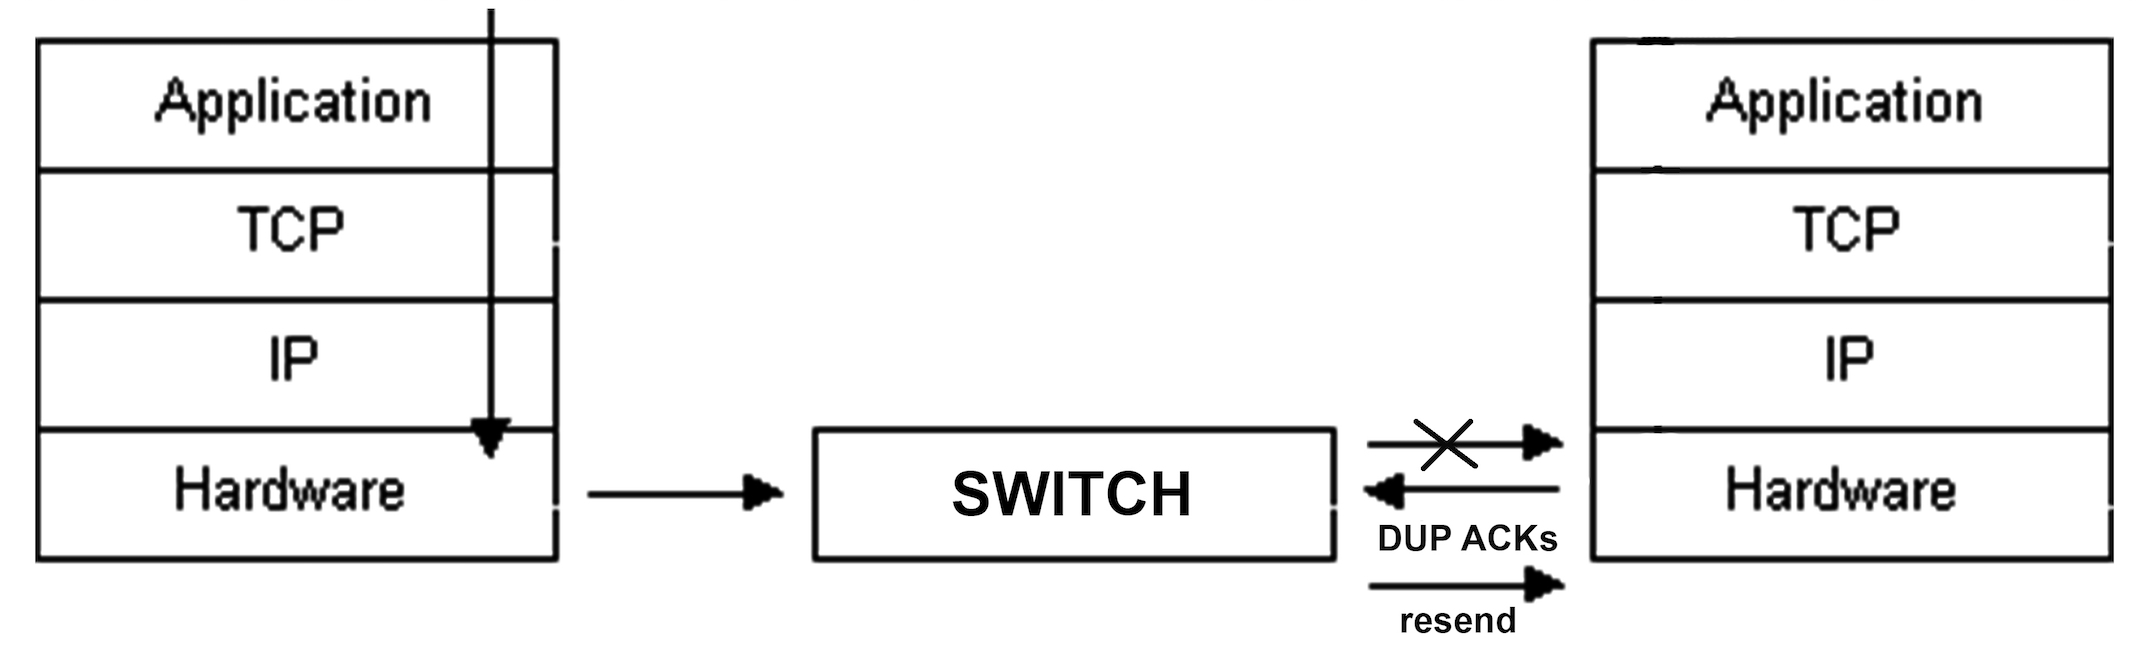
\includegraphics[width=\textwidth]{project-tcp.png}
	\caption{The proposed TCP fast retransmit, assisted by the programmable switch.}
	\label{fig:project-tcp}
\end{figure}
 
This project aims to mitigate last-hop packet drops that are not caused by congestion using a programmable switch. The switch will be able to retransmit the packets from within the network, instead of waiting for the DUP ACKs to get back to the host (Figure \ref{fig:project-tcp}), thereby reduces the response time to DUP ACKs and reduces unnecessary changes to the congestion window. The implementation will be based on the KVS concept, where the keys are the flow ID and the packet sequence number, and the value is the payload.

\section{Related Work}
\label{sec:relate}
\subsection{TCP Congestion Control in Data Centres}
One of the main aspects of TCP is congestion control \cite{rfc2001} where a number of mechanisms are used to achieve high performance and avoid sending more data than the network is capable of forwarding, that is, to avoid causing network congestion. In particular, TCP uses a \textit{congestion avoidance} algorithm that includes various aspects of an additive increase/multiplicative decrease (AIMD) scheme, with other schemes such as \textit{slow start}, \textit{fast retransmit} and \textit{fast recovery} to achieve congestion avoidance. The four intertwined algorithms have been refined over the years and are defined in more detail in RFC 5681 \cite{rfc5681}.

Together with TCP congestion control, there have been a lot of recent researches focusing on mechanisms to handle congestions in the data centres \cite{ecn, dctcp, dcqcn, conga, alizadehattar_et_al:DR:2016:6760} which serve as an inspiration for this project. For instance, Data Center TCP (DCTCP) \cite{dctcp} suggests the use of the Congestion Encountered (CE) code point in the IP header and the ECN-Echo (ECE) flag in the TCP header to allow the sender to compute a congestion estimate and react promptly by reducing the TCP congestion window (cwnd) accordingly.

This project will mostly focus on the \textit{fast retransmit} algorithm, which has been explained in the previous section, and how to assist it using a programmable switch.
\subsection{Programmable Data Planes}
Another key source of inspiration for this project is the emergence of Software-Defined Networking (SDN) \cite{sdn}. The key idea behind it was to physically decouple the control plane from the data plane, which allows centrally managing the control plane in software, while opening the control logic to the users.

In the past, network devices were fixed-function and supported only the functional- ity defined by their manufacturer \cite{sdn}. However, this changes drastically with the introduction of programmable switch-ASICs (Application-Specific Integrated Circuit) \cite{asic} and the rise of SmartNICs. Today, the dominant languages used in this field are P4 \cite{bosshart2014p4, p4spec, p4.org} and Protocol Oblivious Forwarding (POF) \cite{pof, song2013protocol}. They enable faster development/provisioning of new and/or custom protocols, as opposed to the long wait for the release of fixed-function ASIC switches supporting standardised protocols \cite{sivaraman2015dc}.

Different programmable switches have different architectures, but they generally include a programmable pipeline. For example, PISA (Protocol-Independent Switch Architec- ture) is a single pipeline forwarding architecture (Figure \ref{fig:pisa}). The packet is parsed into individual headers. The headers and intermediate results can be used for matching and actions. The headers can also be modified, added or removed. Finally, the packet is deparsed (Figure \ref{fig:pisa1}). This structure has been used in many applications. One of the most popular applications using a programmable switch is In-band Network Telemetry (INT) \cite{int}. It is a framework designed to allow the collection and reporting of network states, by the data plane, without requiring intervention or work by the control plane. The general idea is that packets will contain header fields that are interpreted as “telemetry instructions” by network devices. These instructions tell an INT-programmable device what state to collect and write into the packet as it transits the network. Examples of collectable states are switch id, ingress port id, ingress timestamp or hop latency.

With more focus, data plane programmability has the potential to benefit future-proof forwarding devices, which are able to support major control plane and protocol updates, without mandating any hardware upgrades.
